\chapter{FEM modelisation}

In classical FEM, typically the elements are constructed from Lagrange polynomials, known as Lagrange elements, where the interpolating polynomials define unity at the nodes. This property means that the nodes lie on the surface discretised by Lagrange elements, which brings the intuition of Node-to-Node contact where the contact is defined between the nodes of conforming meshes at the contact interface. 
Node-to-Node contact can be essentially considered as the collocation method where the strong form of contact or friction definition is satisfied at the nodes in $\Gamma_C$. The area effects can also be partly considered through Isoparametric mapping even though it may not be precise.\\


\iffalse
Even though the factor $c_n$ in the contact integral is determined experimentally in the light of normal compliance approach, the characteristics of  depends on the underlying numerical formulation.

There are some strategies which adapt the collocation scheme to take in to account of area implicitly, where typically contact pressure is correlated to contact stiffness or experimentally determining contact stiffnesses across the contact interface. 
With the former approach of correlating contact stiffness to contact pressure, the contact pressure solved from $\bm{u}_{eq}$ can also be considered as the correlation factor to define contact stiffness for $\bm{\widetilde{u}}$.\\
\fi

Given that we focus on shape optimisation, Node-to-Node contact can place severe constraints in meshing, where structured meshing must be preferred to define confirming meshes at the contact interface. Depending on the design space in shape optimisation, this may not be a very robust strategy, since structured meshing can severely restrict mesh adaptation to avoid distorted elements that can effect the Isoparametric definition of integrals. 
On the other hand, it is well known that unstructured mesh definition may not also lead to robust meshing with classical FEM. 
Due to such complications with meshing, Isogeometric approach can be considered by choosing a robust parameterization strategy which would be rather difficult with classical FEM. 
But also the Node-to-Node contact can not be explicitly defined with Isogeometric approach, since the control points which correspond to nodes in classical FEM may not lie on the surface. 
Rather, the collocation may not have to be on the nodes which is typically preferred in classical FEM, but else where on the surface. 
Hence, the collocation scheme in classical FEM typically defined with Node-to Node contact takes a different form with Isogeometric approach, where the collocation can be defined on the surface or implicitly in the knot span.
We also remind that defining an initial Parametrisation may also be cumbersome with Isogeomtric approach but given a well-defined initial parameterisation, Isogeometric approach can achieve robust refinement.
Although the complications with meshing for classical FEM can be avoided with contact formulations that do not demand confirming meshes at the interface, developing such formulations with Isogeometric approach can be even more advantageous in shape optimisation.\\ 

The effect of contact formulation to the prediction of instabilities with CEA has not been largely studied, where the interest is on the contact characteristics pertaining to the dynamics of the perturbation $\bm{\widetilde{u}}$ rather than $\bm{u}_{eq}$ \eqref{pert_wrt_eq}. 
Nevertheless, we develop a more rigorous formulation with Isogeometric approach in {\color{red} \S}, purely for its advantages in optimisation, where it does not require confirming meshes at the interface -- since also defining confirming meshes can be even more cumbersome with Isogeometric approach due to the tensor product nature of NURBS.\\

We define optimisation of simple shapes through classical FEM discretisation, where the definition of simple shapes vow for a robust structured meshing and hence Node-to-Node contact can be preferred for its simplicity.
With the following explanations, we detail the Node-to-Node collocation method to model the contact and the friction definitions in the problem \eqref{pert_dyn}, where we also show the relation of collocation method to the weak form of contact and friction terms in  \eqref{weak_pert_2}. 
It should be noted that this type of contact and friction definitions are defined with approximations specific for modelling flutter-type dynamic instability with CEA, detailed in {\color{red}\S}.
Considering Eq. \eqref{weak_pert_2}, for classical FEM with Lagrange elements, the space ${}_h \bm V$ is defined by the bases $ {}_h \bm v_i $ of Lagrange polynomials.  





\subsubsection{Contact formulation} \label{weak_pert_2}

The contact definition of the initial-boundary value problem Eq. \eqref{pert_dyn} can be defined in finite element context as

\begin{equation}
{}_h\sigma^{(\mathrm k)}_n({}_h\bm{\widetilde u}^\mathrm{(k)}) = - \mathit{p}{{}_h\widetilde{u}_n}^{(\mathrm k)} \quad \mathrm{on}\quad\Gamma^{\mathrm{(k)}}_C\\
\end{equation}

where for a system with two domains $\Omega^{(a)}$ and  $\Omega^{(b)}$ in contact. 
With confirming mesh at $\Gamma_C^{(a)}$ and $\Gamma_C^{(b)}$, it can be said that for any node ${i} \in \Gamma_C^{(\mathrm a)}$, there exists a unique node ${j} \in \Gamma_C^{(\mathrm b)}$ that forms contact. Hence, the contact force for a given node $i \in \Gamma_C^{\mathrm (a)}$ in contact with a node $j \in \Gamma_C^{\mathrm (b)}$ can simply be expressed with Node-to-Node contact as

\begin{equation}
  \mathit{p}({{}_h\widetilde{\bm u}}^{(\mathrm a)} - {{}_h \widetilde{\bm u}}^{ ( \mathrm b)}). \bm{\hat{\mathrm v}}_n\bigg|_{ {}_h \bm v_i^\mathrm{(a)}= {}_h \bm v_i^\mathrm{(b)}=1}  = p ( \widetilde{ \bm u}_{{i}}^{(\mathrm a)}- \widetilde{ \bm u}_{{j}}^{(\mathrm b)}). \bm{\hat{\mathrm v}}_n = {}_ht^{(\mathrm k)}_n
\end{equation}

where ${{}_h\widetilde{\bm u}}^{(\mathrm a)} = \sum_{\forall {i} \in \Omega^{(\mathrm a)}} {}_h\bm v_i^\mathrm{(a)} \widetilde{\bm u}_i^\mathrm{(a)}$ and ${{}_h\widetilde{\bm u}}^{(\mathrm b)} = \sum_{\forall {j} \in \Omega^{(\mathrm b)}} {}_h\bm v_j^\mathrm{(b)} \widetilde{\bm u}_j^\mathrm{(b)}$. Since the collocation is defined at the nodes itself, the bases ${}_h \bm v_i^\mathrm{(a)}= {}_h \bm v_i^\mathrm{(b)}=1$ for Lagrange elements or typically for elements in classical FEM. The above equation is stated specifically for linear case, where normal compliance terms are expressed to be linear.\\

As an alternate interpretation, the collocation method can also be defined from the weak form of contact \eqref{pert_cont} as

\begin{multline}
{\langle {}_h \bm{\sigma}^{\mathrm{(a)}}_n, {}_h \bm v_i^\mathrm{(a)} \rangle_{\Gamma_C^{\mathrm{(a)}}}} =\int_{\Gamma^{(a)}_C}  \mathit{p}[({{}_h\widetilde{\bm u}}^{(\mathrm a)} - {{}_h \widetilde{\bm u}}^{ ( \mathrm b)}). \bm{\hat{\mathrm v}}_n]  {}_h \bm v_i^\mathrm{(a)}. \bm{\hat{\mathrm v}}_n \,\,d{\Gamma^{(\mathrm a)}_C}
\rightarrow\\ 
p ( \widetilde{ \bm u}_{{i}}^{(\mathrm a)}- \widetilde{ \bm u}_{{j}}^{(\mathrm b)}). \bm{\hat{\mathrm v}}_n\end{multline}

if the weighting function $ {}_h \bm v_i^\mathrm{(a)}$ of the weak form is defined to be the Dirac-delta function $(\delta_D(.))$ as $ {}_h \bm v_i^\mathrm{(a)} = \delta_D(\widetilde{ \bm u}_{{i}}^{(\mathrm a)} - \widetilde{ \bm u}^{(\mathrm a)})$ \footnote{$ \delta_D(\widetilde{ \bm u}_{{i}}^{(\mathrm a)} - \widetilde{ \bm u}^{(\mathrm a)}): {}_h \bm v_i^\mathrm{(a)} = 0, \,\, \forall \widetilde{ \bm u}_{{i}}^{(\mathrm a)} \neq \widetilde{ \bm u}^{(\mathrm a)}$ and ${}_h \bm v_i^\mathrm{(a)} = 1$ if $\widetilde{ \bm u}_{{i}}^{(\mathrm a)} = \widetilde{ \bm u}^{(\mathrm a)}$}.\\


As aforementioned, we do not focus on the physical characteristics of contact stiffness in the light of normal compliance, and its subsequent effect on CEA, where we define contact stiffness purely as a penalty coefficient $p$. 
But to proceed with the following discussions, we must make a strong assumption on the existence of global contact stiffness ($p_{G}$) such that this property is independent of the contact interface area. 
This is because, if $p$ is a parameter of differential area determined from experiments, it cannot be taken in to account with Node-to-Node contact unless area is implicitly considered. This is largely the case if contact stiffness has correlation with contact pressure at the interface. 
%This is also important to eliminate bias of contact stiffness in optimisation. 
%With this assumption, This is to eliminate bias in optimisation, where larger area can have larger contact stiffness globally relative to a shape with smaller contact area. 
%Hence, we implicitly make a strong assumption that contact stiffness is property associated globally. 
%This can also be interpreted as $p_{G}$  being associated with net force, while local contact stiffness ($p_{l}$) being associated with pressure, which may not be necessarily true.  
 It is only safe to say that experimental studies can alone determine if $p$ is a global or local parameter, such that to eliminate any bias of contact stiffness in defining instability for shape optimisation. 
Nevertheless, with this strong proposition, contact stiffness between any two spatially corresponding nodes is defined by local contact stiffness $p_{l}$, defined as 
   
\begin{equation}
p_{l} = \frac{p_G}{\mathrm{m}}
\end{equation}\\

where ${\mathrm{m}}$ is the number of contact nodes at the interface.
%The convergence of the stability criteria $C_s$ for a given design point based on the choice of the number of contact pairs is also discussed in \S.\\

Similarly, the friction definition of the initial-boundary value problem Eq. \eqref{pert_dyn} can be defined in finite element context as 

\begin{equation}
{}_h\sigma^{(\mathrm k)}_t({}_h\bm{\widetilde u}^\mathrm{(k)}) = \mu \mathit{p}{{}_h\widetilde{u}_n}^{(\mathrm k)} \quad \mathrm{on}\quad\Gamma^{\mathrm{(k)}}_C\\
\end{equation}

Similar to the definition of contact force, the tangential force of friction can be defined with Node-to-Node collocation as 

\begin{equation}
  \mu \mathit{p}({{}_h\widetilde{\bm u}}^{(\mathrm a)} - {{}_h \widetilde{\bm u}}^{ ( \mathrm b)}). \bm{\hat{\mathrm v}}_n\bigg|_{ {}_h \bm v_i^\mathrm{(a)}= {}_h \bm v_i^\mathrm{(b)}=1}  = \mu p ( \widetilde{ \bm u}_{{i}}^{(\mathrm a)}- \widetilde{ \bm u}_{{j}}^{(\mathrm b)}). \bm{\hat{\mathrm v}}_n
\end{equation}

where vectorially, the friction force can be expressed as $\mu [p ( \widetilde{ \bm u}_{{i}}^{(\mathrm a)}- \widetilde{ \bm u}_{{j}}^{(\mathrm b)}). \bm{\hat{\mathrm v}}_n]\bm{\hat{\mathrm v}}_t$, with $\bm{\hat{\mathrm v}}_t$ for a given node being known a priori. For the $d-p$ system, the friction force can be resolved in to tangential and radial components relative to the disc axis. Since, the relative sliding velocity is negligible in the radial direction, the frictional force component of the radial direction is also negligible and hence often ignored. 

\iffalse
\subsubsection{Model reduction}

The evaluation of the stability criterion $C_s$ involves expensive computation for eigenvalues evaluated at various friction coefficients to capture the evolution of the instability. While only the major unstable modes constituting the squeal noise is required to be identified, the model can be simplified by dynamic model reduction techniques. This further allows us to simplify the damping definition of the dynamic model with the method of modal damping. The method of Craig \& Bampton reduction is applied to the model, which is considered to be effective since it captures the dynamic properties at the contact interface and also the internal dynamic properties of the models involved in contact. More detailed description of Craig \& Bampton method used in brake squeal application can be found in literature \cite{BESSET2017896} and \cite{MONTEIL20161073}.   In accordance with the Craig \& Bampton theory,

\begin{equation}
\bm U=\left\{
\begin{array}{c}
     {\bm U}_i  \\
     {\bm U}_j 
\end{array}\right\};
\quad
\bm K=\left[
\begin{array}{cc}
  {\bm K}_{ii} &{\bm K}_{ij} \\
  {\bm K}_{ji} &{\bm K}_{jj} \\
\end{array}
\right];
\quad
\bm M=\left[
\begin{array}{cc}
  {\bm M}_{ii} &{\bm M}_{ij} \\
  {\bm M}_{ji} &{\bm M}_{jj} \\
\end{array}
\right]
%\left[
%\begin{array}{cc}
%{\bm U_i}\\
%{\bm U_j}\\
%\end{array}
%\right]
%=
%\left[
%\begin{array}{cc}
%F_i\\
%F_j\\
%\end{array}
%\right]
\end{equation}\\

where $\bm U_i$ and $\bm U_j$ are internal and interface degrees of freedom respectively. The transformation matrix $\bm T$ is defined as composition of static transformation ${\bm \Phi}_s$ and Eigen vectors ${\bm \Phi}_d$, as follows\\

\begin{equation}
{\bm T}=
\left[
\begin{array}{cc}
  {\bm \Phi}_d &{\bm \Phi}_s \\
  \bm 0 & \bm I \\
\end{array}
\right];
\quad
{\bm\Phi}_s={\bm K}_{ii}^{-1} {\bm K}_{ij};
\quad
{\bm \Phi}_d=[\Phi_0,\Phi_1,...,\Phi_n]\
\end{equation}\\


where $\Phi_n$ is the $n^\text{th}$ eigenvector obtained from the eigenvalue problem defined as $({\bm K}_{ii}-\omega_n^2{\bm M}_{ii})\Phi_n=0$. The choice of the number of eigenvectors $n$ considered for reduction depends on the convergence required with respect to prediction of the eigenvalues for the unstable modes obtained by the reduced model.\\

The reduced mass matrix ${\bm  M}_{r}$ and stiffness matrix ${\bm  K}_{r}$ are respectively obtained through the transformation matrix ${\bm T}$ applied as ${\bm T}^t{\bm  M}_{s}{\bm T}$ and ${\bm T}^t{\bm  K}_{s}{\bm T}$, where ${\bm  K}_{s}$ is the stiffness matrix of the system with friction definition. The matrix ${\bm  K}_{r}$ is largely uncoupled, defined in the modal coordinates, except for the non-diagonal terms which can be viewed as the terms constituting the effects of friction in the modal coordinates and also the part of the matrix with static reduction is non-diagonal. While the reduction of the mass matrix from ${\bm  M}_{s}$ to ${\bm  M}_{r}$ is simply straight forward.\\

The Craig-Bampton reduction leads to reduced matrices of size ${\bm[\;S\times S\;]}$, where $\bm S$ is given by the sum of the number of contact points at the system interface and the number of eigenvectors of the system considered. This greatly reduces the computation time of the Complex eigenvalue analyses for the estimation of the stability criteria. \\

\fi


\subsubsection{Mesh sensitivity}

In relation to the expensive evaluation of the stability criteria, mesh convergence study was performed for the influence of mesh at the contact interface and outside the contact interface. The eigenmodes reflecting maximum instability as predicted by the maximum positive real part of the complex eigenvalues are only of interest to us and hence taken in to account to check for convergence. It should be noted that the contact formulation can have some influence on mesh convergence especially for CEA, where no clear studies has been performed. In this case, we are specific for convergence with for node-to-node formulation. \\

The dynamic properties with respect to maximum instability show little variation for change in mesh size out of the contact region for a given shape and number of contact points. The comparison is shown through a model with highly coarse mesh as in Fig. \ref{fig:coarse_mesh} against  a model with the same shape but for a relatively fine mesh as in Fig. \ref{fig:h_mesh}, while maintaining the same number and position for the contact points. The mismatch in frequencies between the models is shown in Fig. \ref{fig:h_freq} where the range for frequency is zoomed to a pair of frequencies which induce mode coalescence predicted to cause the maximum instability. The shift in unstable frequencies and the point of bifurcation of the maximum real part as shown in Fig. \ref{fig:h_real} are observed to be very low for change in mesh size.\\


\begin{figure}
    \centering
    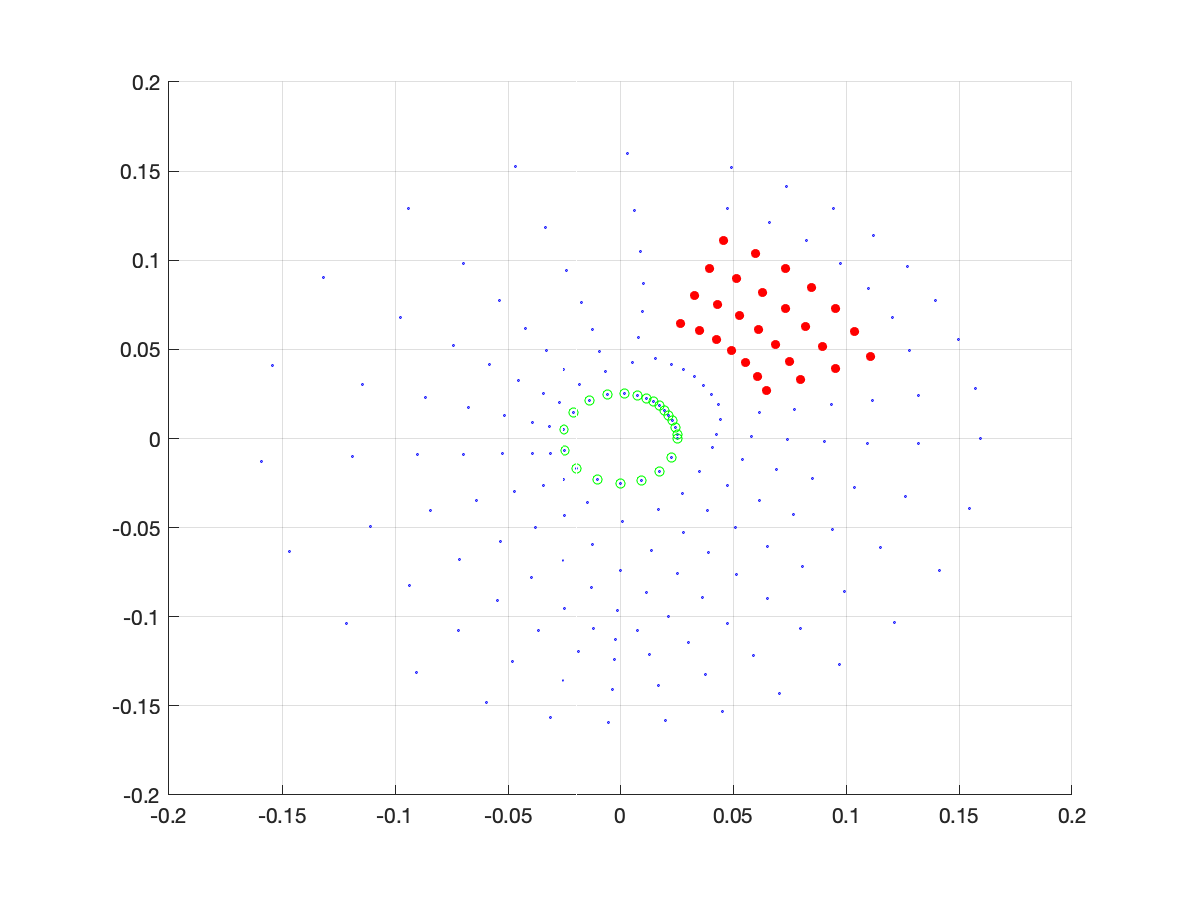
\includegraphics[scale=0.43]{Chapter2/Pictures/Geo_pub_h1.eps}
    \caption{Node plot for a coarse mesh of the disc geometry with contact nodes represented in red}
    \label{fig:coarse_mesh}
\end{figure}

\begin{figure}
    \centering
    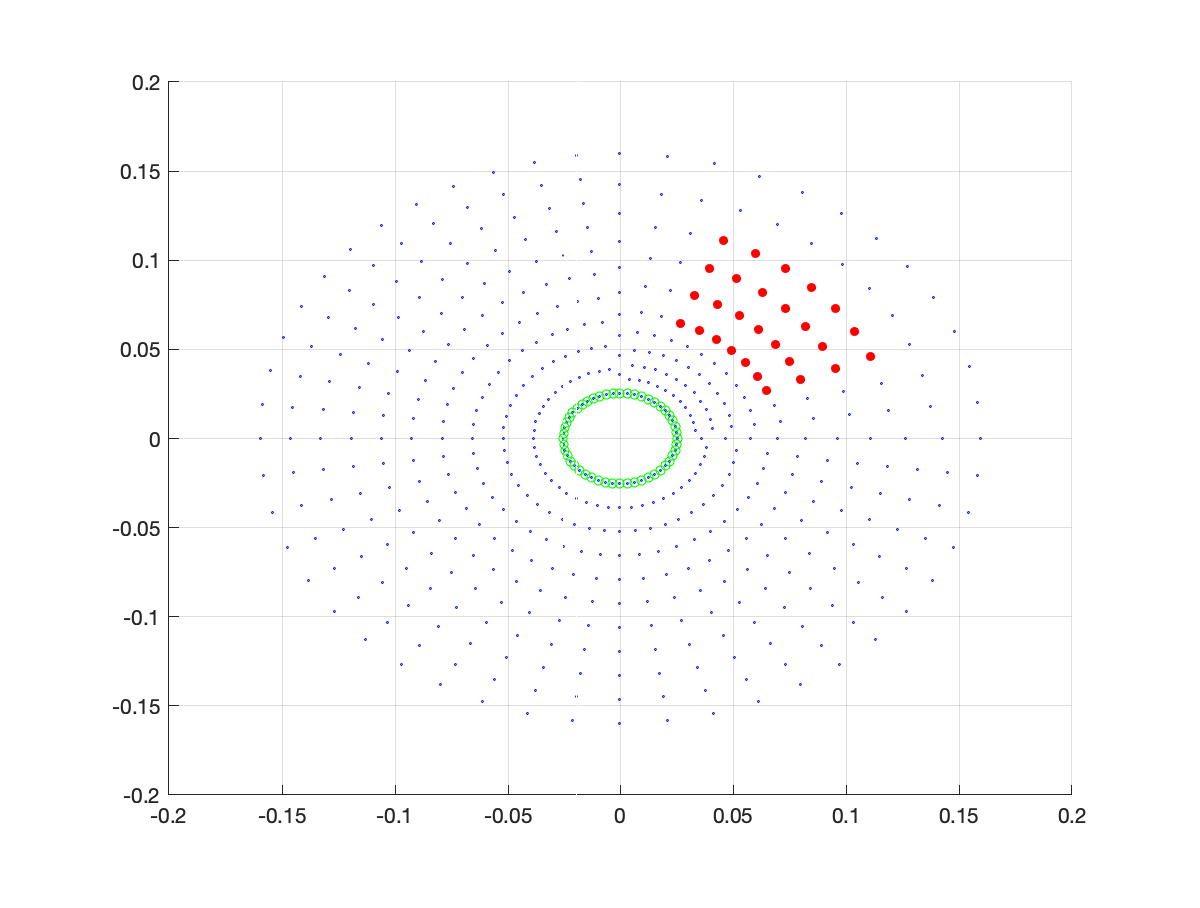
\includegraphics[scale=0.43]{Chapter2/Pictures/Geo_pub_h.eps}
    \caption{ Node plot for a relatively fine structured mesh of the disc geometry with contact nodes represented in red}
    \label{fig:h_mesh}
\end{figure}

\begin{figure}
    \centering
    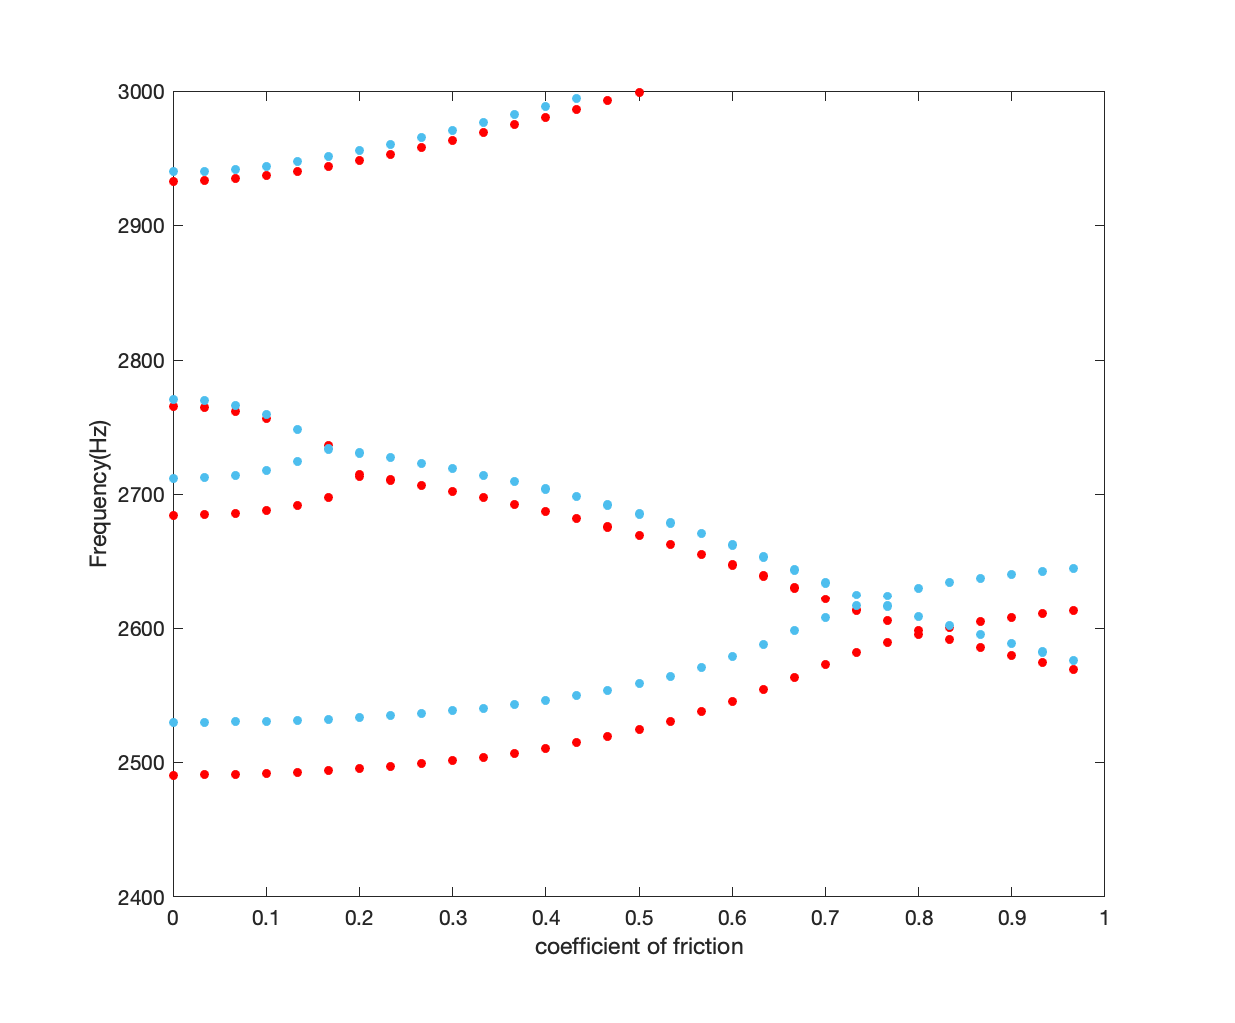
\includegraphics[scale=0.43]{Chapter2/Pictures/hvsh1_freq1.eps}
    \caption{Plot of Frequency vs Friction coefficient, of modes showing maximum instability; Blue represents for the model in \ref{fig:coarse_mesh}; Red represents for the model in \ref{fig:h_mesh}}
    \label{fig:h_freq}
\end{figure}

\begin{figure}
    \centering
    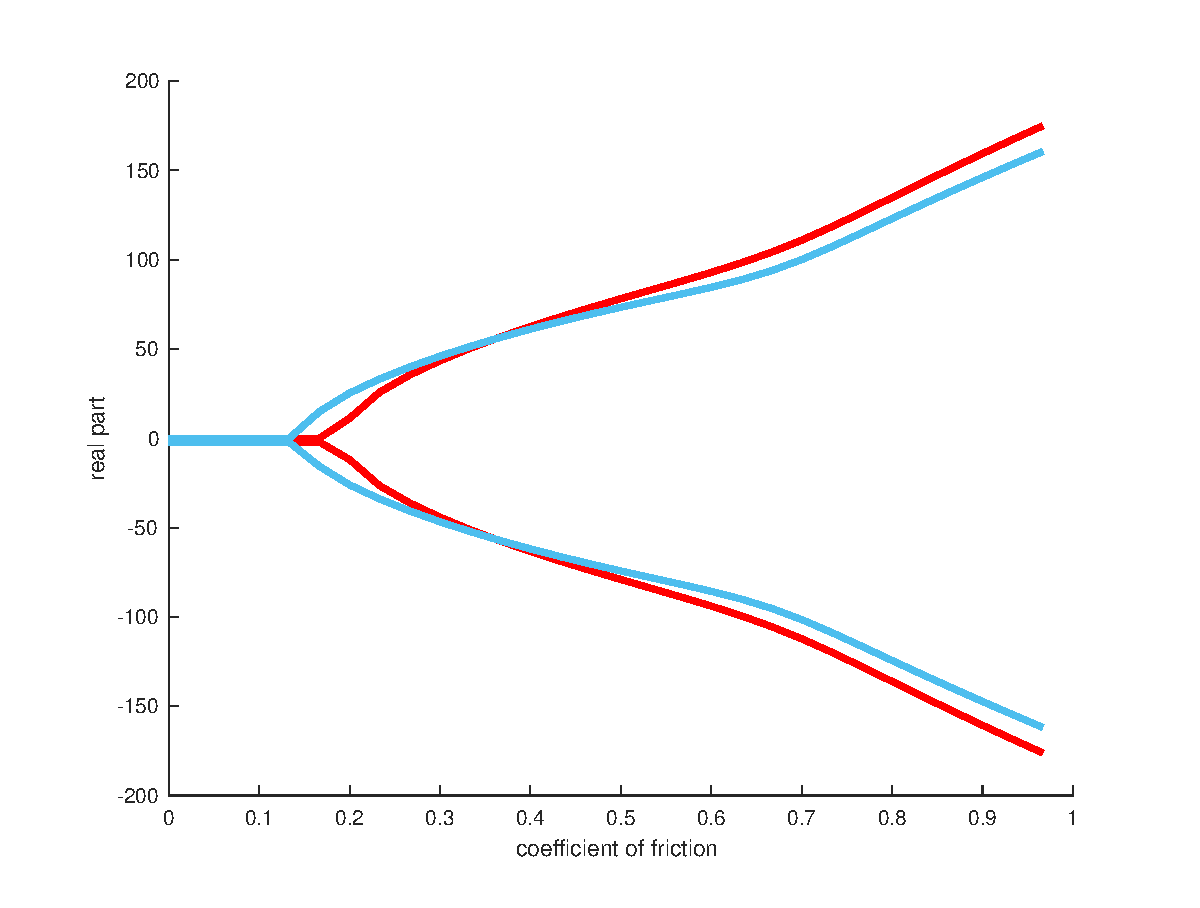
\includegraphics[scale=0.43]{Chapter2/Pictures/hvsh1_real.eps}
    \caption{Plot of Real part of the complex eigenvalues vs Friction coefficient, of modes showing maximum instability; Blue represents for the model in \ref{fig:coarse_mesh}; Red represents for the model in \ref{fig:h_mesh}}
    \label{fig:h_real}
\end{figure}

Though the variation of the mesh out of the contact interface is shown to have a little influence on the maximum instability, the variation of mesh at the contact interface is observed to have a considerable effect on the dynamic properties. This can be seen by comparing results of the models in Fig. \ref{fig:coarse_mesh} and Fig. \ref{fig:h_mesh} against the models in Fig. \ref{fig:hh_mesh} and Fig. \ref{fig:hhhh_mesh} which are of the same shape. Hence, it is intuitive to assume a large number of contact points, since the contact interface is a continuum after all. The convergence is shown with large number of contact points in Fig. \ref{fig:hh_mesh} and Fig. \ref{fig:hhhh_mesh} with plot for bifurcation of the real part in Fig. \ref{fig:hhhh_real}) and frequencies inducing maximum instability in Fig. \ref{fig:hhhh_freq}. \\

\begin{figure}
    \centering
    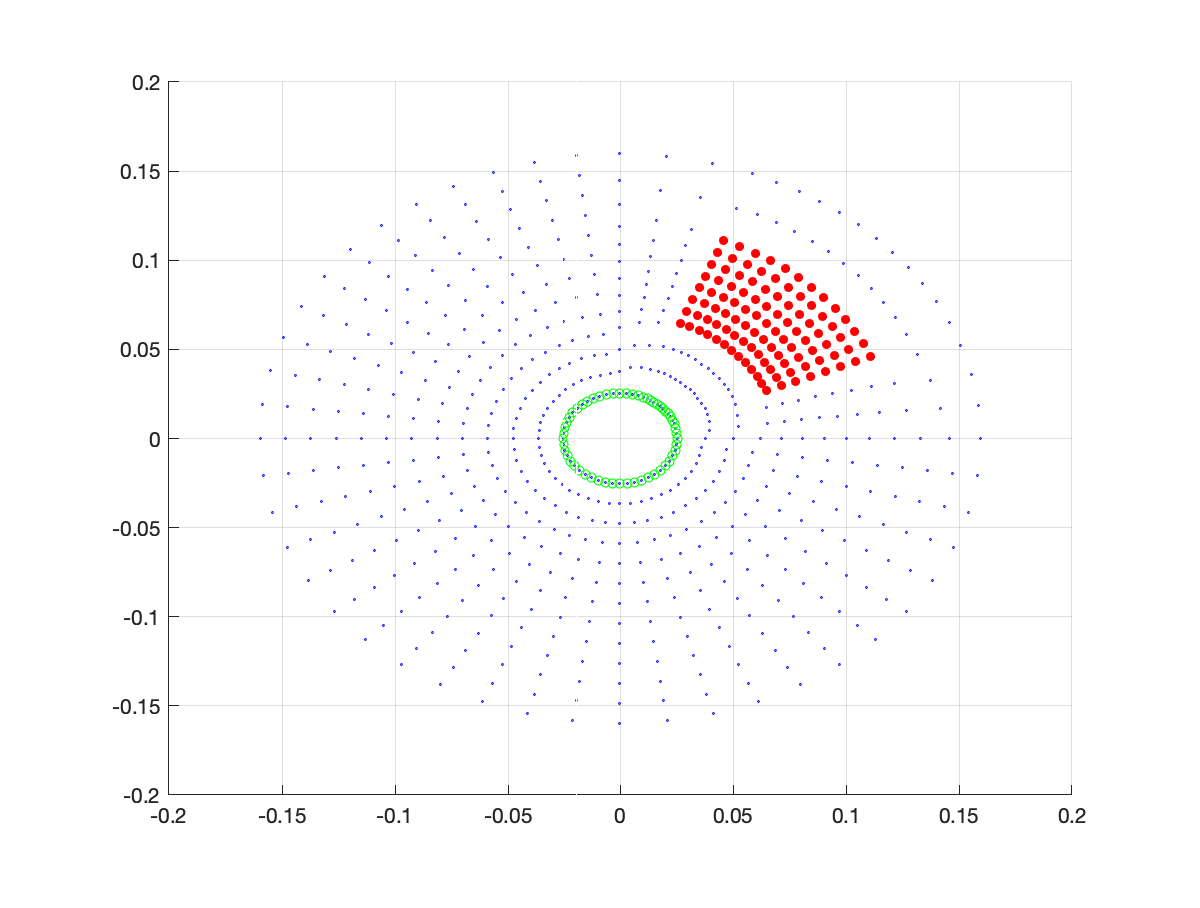
\includegraphics[scale=0.43]{Chapter2/Pictures/Geo_pub_hh.eps}
    \caption{Node plot for a fine mesh with contact nodes represented in red}
    \label{fig:hh_mesh}
\end{figure}

\begin{figure}
    \centering
    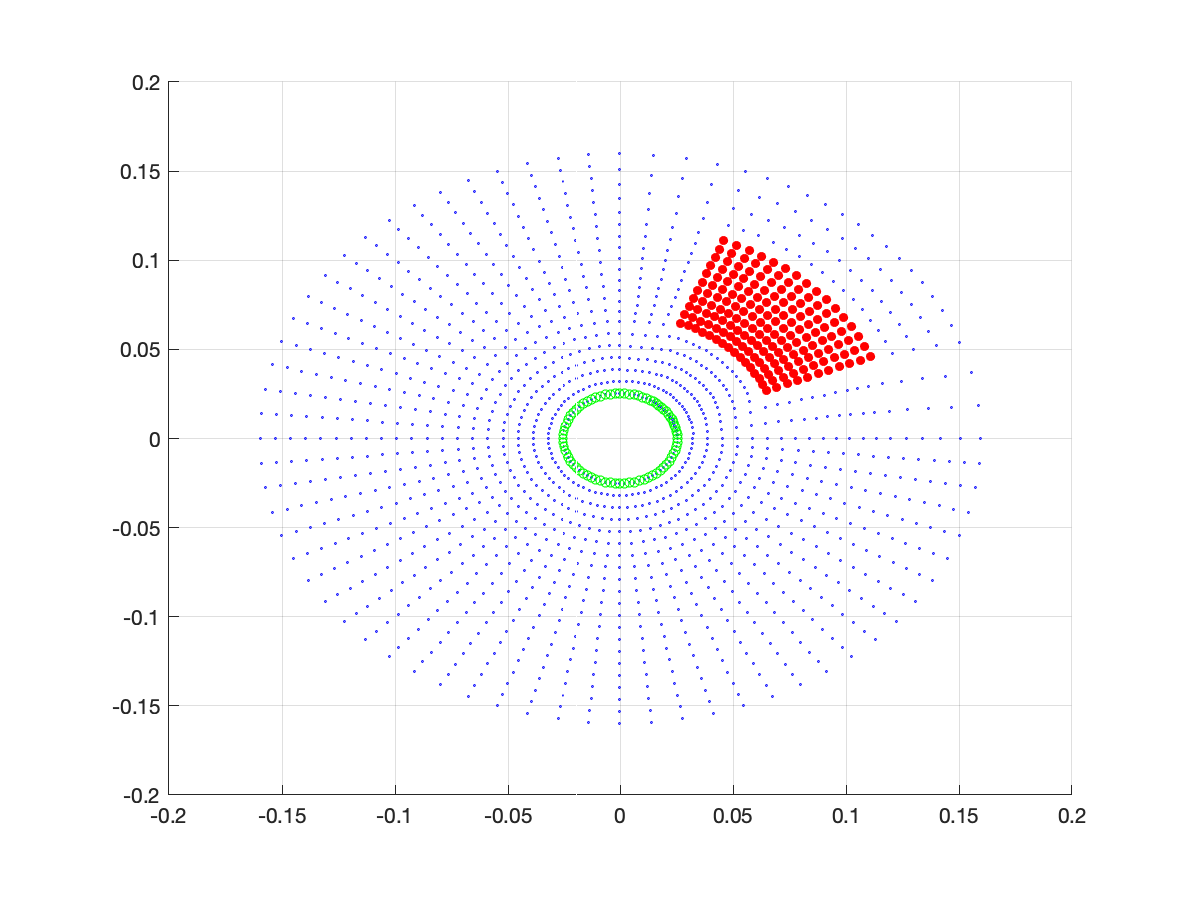
\includegraphics[scale=0.43]{Chapter2/Pictures/Geo_pub_hhhh.eps}
    \caption{ Node plot for a relatively finer mesh compared to \ref{fig:hh_mesh}, especially on the contact interface with contact nodes represented in red}
    \label{fig:hhhh_mesh}
\end{figure}

\begin{figure}
    \centering
    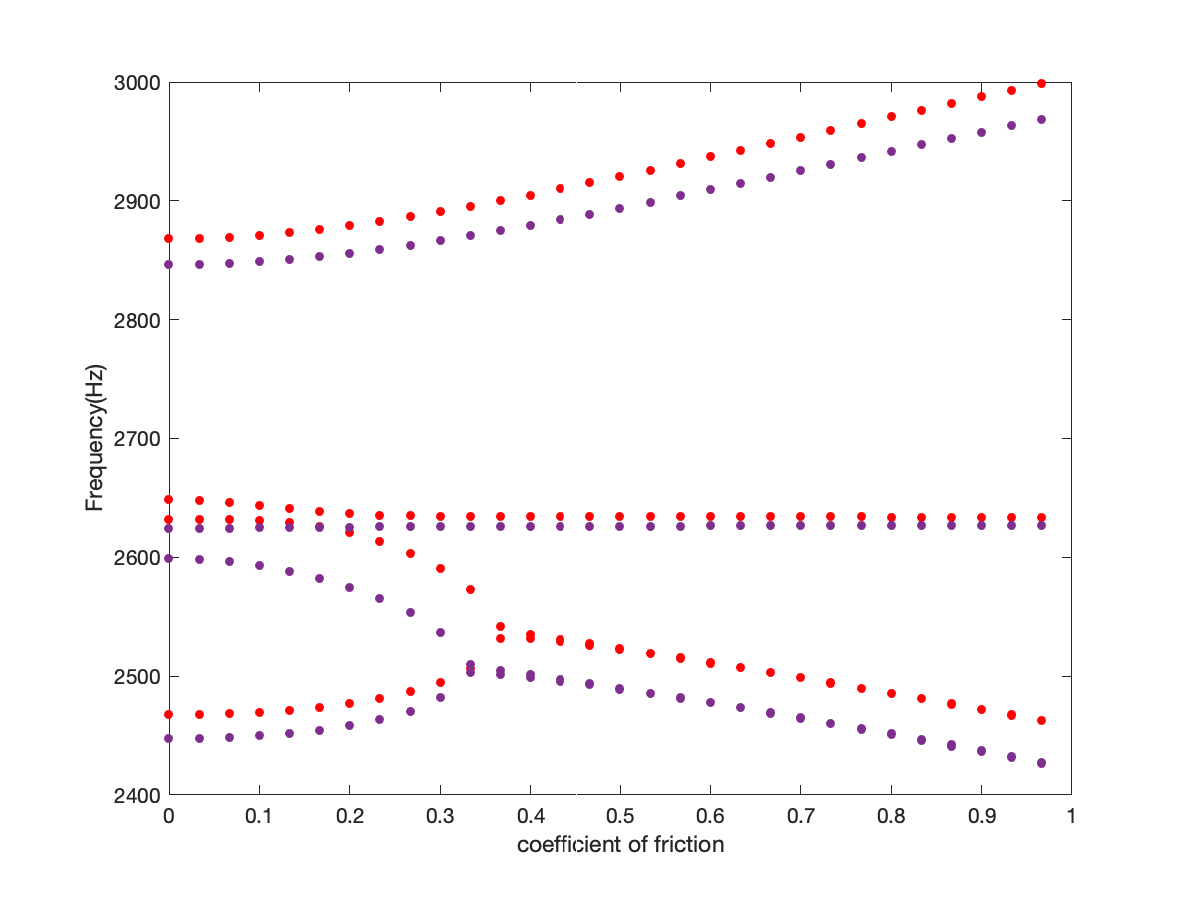
\includegraphics[scale=0.43]{Chapter2/Pictures/hhvshhhh_freq.eps}
    \caption{Plot of Frequency vs Friction coefficient, of modes showing maximum instability; Red represents the plot for the model in \ref{fig:hh_mesh}; Violet represents the plot for the model in \ref{fig:hhhh_mesh}}
    \label{fig:hhhh_freq}
\end{figure}

\begin{figure}
    \centering
    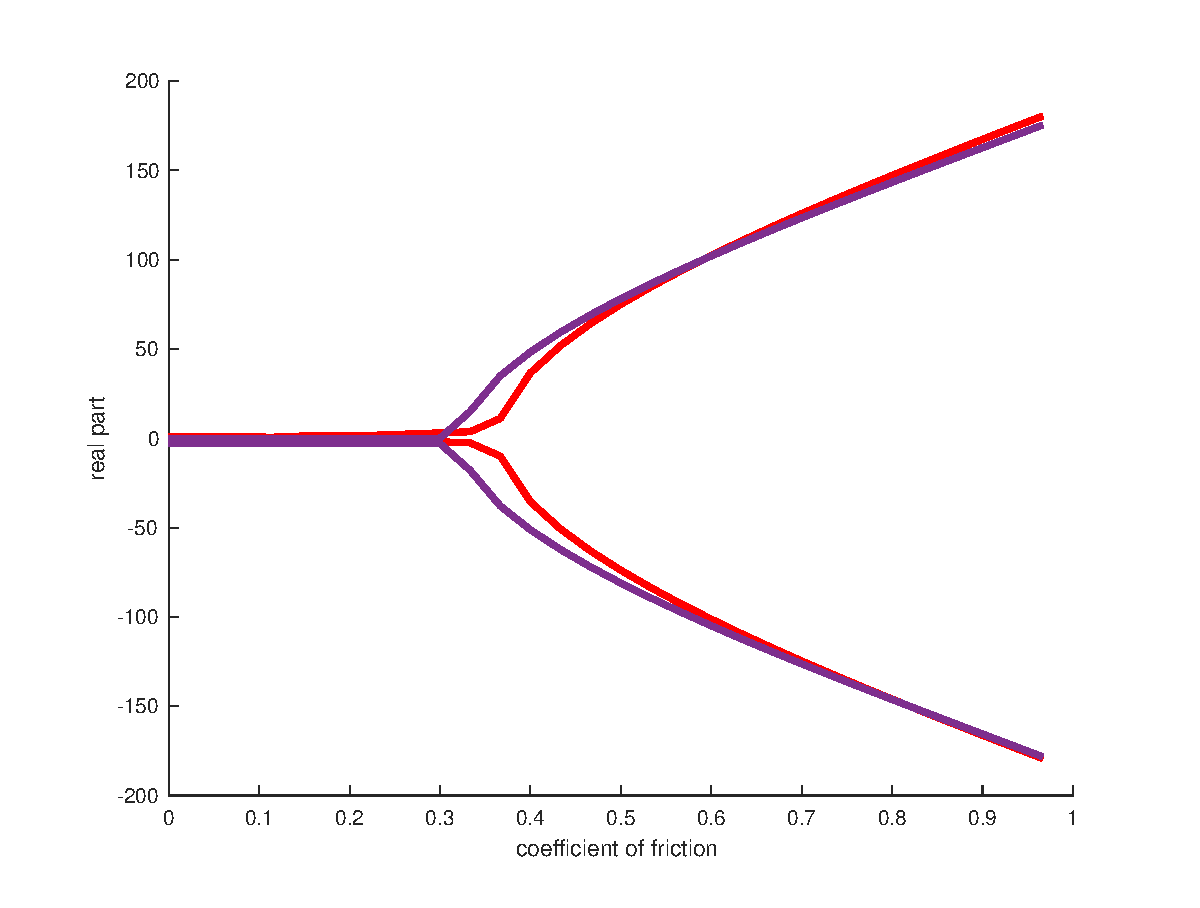
\includegraphics[scale=0.43]{Chapter2/Pictures/hhvshhhh_real.eps}
    \caption{Plot of Real part of the complex eigenvalues vs Friction coefficient, of modes showing maximum instability; Red represents the plot for the model in \ref{fig:hh_mesh}; Violet represents the plot for the model in \ref{fig:hhhh_mesh}}
    \label{fig:hhhh_real}
\end{figure}

The definition of the contact points can be observed to have significant influence on the maximum real part of the complex eigenvalues and hence also the stability criteria, which demands a good mesh definition to define a robust stability criteria in optimisation. For this reason, we defined a structured mesh as in Fig. \ref{fig:disc_mesh} where linear hexahedral elements are largely used through out the model with smaller elements at the contact interface, while the region outside of contact interface is defined by larger elements. The difference in mesh density is compromised by introducing 3D wedge elements to maintain a structured mesh.\\ 


\begin{figure}
    \centering
    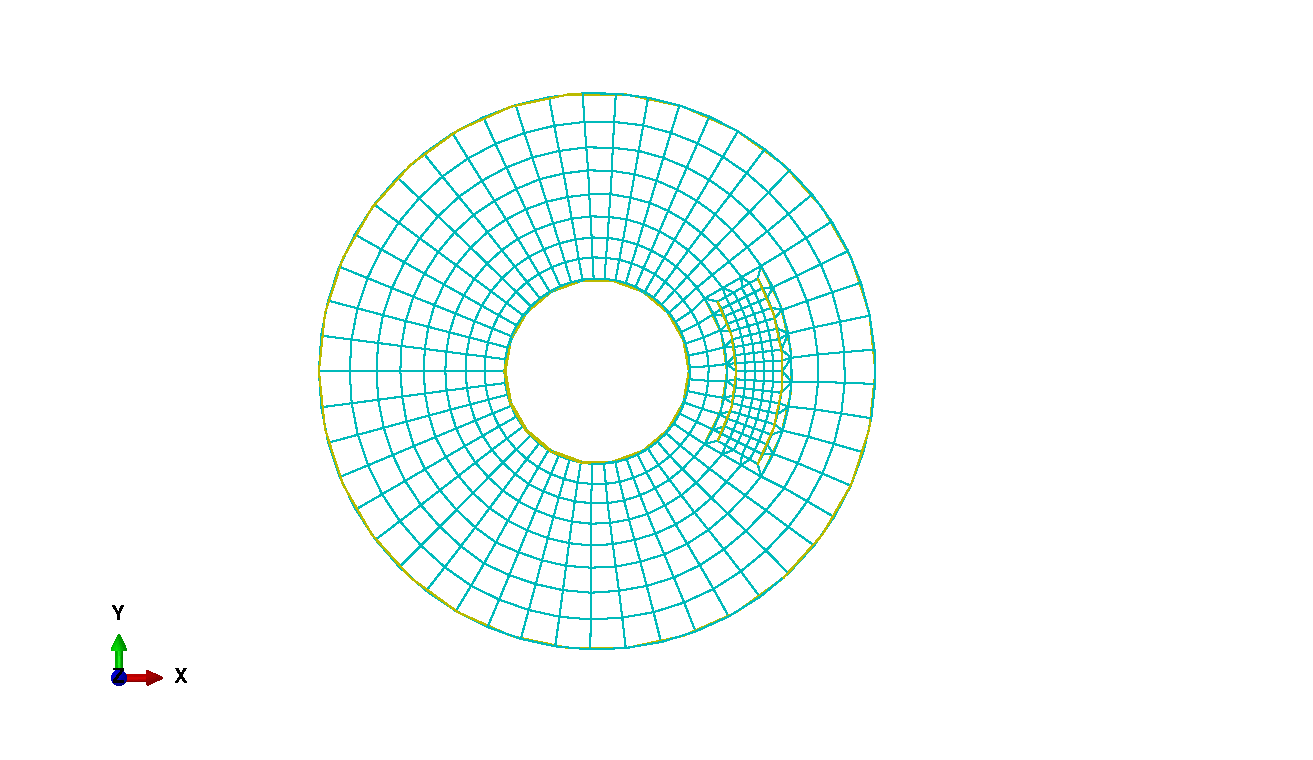
\includegraphics[scale=0.6]{Chapter2/Pictures/disc1.eps}
    \caption{Considered mesh definition}
    \label{fig:disc_mesh}
\end{figure}





